\documentclass[11pt,reqno,final]{amsart}

\pdfcompresslevel=0
\pdfobjcompresslevel=0

\usepackage[dvipsnames]{xcolor}% adds colors
\usepackage{amsmath, amsthm}% {amsfonts, amssymb}

% New Characters
\usepackage[latin1]{inputenc}%
\usepackage[T1]{fontenc}

\usepackage{MnSymbol}
\usepackage[normalem]{ulem}% underlining

\usepackage[theoremfont, largesc]{newpxtext} % different text,math font
\usepackage{newpxmath}

\makeatletter
\DeclareMathRadical{\sqrtsign}{symbols}{112}{largesymbols}{112}
% \let\sqrt=\undefined
% \DeclareRobustCommand\sqrt{\@ifnextchar[\@sqrt{\mathpalette\@x@sqrt}]}
% \def\@x@sqrt#1#2{%
%  \setbox\z@\hbox{$\m@th#1\sqrtsign{\mkern1mu #2}$}
%  \mkern3mu\box\z@}
\makeatother




% Page Typesetting
\usepackage[final]{microtype}
\usepackage{relsize}
\usepackage[margin=1in]{geometry}
\usepackage{framed}
\usepackage{tikz}

\usepackage{csquotes}

\usepackage{setspace}
\onehalfspacing

\usepackage{hyperref}
\hypersetup{
  final,
  pdftitle={Math 135 - Extreme Values},
  pdfauthor={Bonventre}, 
  linktoc=page,
  pagebackref,
  colorlinks=true,
  citecolor=PineGreen,
  linkcolor=PineGreen,
  linkbordercolor=PineGreen,
}


% Internal References

\usepackage[inline,shortlabels]{enumitem}

% \numberwithin{equation}{section} 
\numberwithin{figure}{section}

\usepackage[nameinlink,capitalise,noabbrev]{cleveref}

\crefname{equation}{}{} % get \cref to behave as \eqref

% \theoremstyle{plain} % bold name, italic text
\newtheorem{theorem}[equation]{Theorem}%
\newtheorem*{theorem*}{Theorem}%
\newtheorem{lemma}[equation]{Lemma}%
\newtheorem{proposition}[equation]{Proposition}%
\newtheorem{corollary}[equation]{Corollary}%
\newtheorem{conjecture}[equation]{Conjecture}%
\newtheorem*{conjecture*}{Conjecture}%
\newtheorem{claim}[equation]{Claim}%
\newtheorem{question}{Question}

\theoremstyle{definition} % bold name, plain text
\newtheorem{definition}[equation]{Definition}%
\newtheorem*{definition*}{Definition}%
\newtheorem{example}[equation]{Example}%
\newtheorem*{example*}{Example}%
\newtheorem{remark}[equation]{Remark}%
\newtheorem{notation}[equation]{Notation}%
\newtheorem{convention}[equation]{Convention}%
\newtheorem{assumption}[equation]{Assumption}%
\newtheorem{exercise}[question]{Exercise}

% ---------- macros
\newcommand{\set}[1]{\left\{#1\right\}}%
\newcommand{\sets}[2]{\left\{ #1 \;|\; #2\right\}}%
\newcommand{\longto}{\longrightarrow}%
\newcommand{\into}{\hookrightarrow}%
\newcommand{\onto}{\twoheadrightarrow}%

\usepackage{harpoon}
\newcommand{\vect}[1]{\text{\overrightharp{\ensuremath{#1}}}}

\newcommand{\del}{\partial}%

\newcommand{\ki}{\chi}
\newcommand{\ksi}{\xi}
\newcommand{\Ksi}{\Xi}

\newcommand{\dlim}{\displaystyle\lim}

% %%%%%%%%%%%%%%%%%%%%%%%%%%%%%%%%%%%%%%%%%%%%%%%%%%%%%%%%%%%%%%%%%%%%%%%%%%%%%%%%%%%%%%%%%%%%%%%%%%%%

\begin{document}


\begin{center}
        \textbf{\Large Math 135, Calculus 1, Fall 2020}\\[10pt]
        {\large 11-09: Extreme Values (Section 4.2)}
\end{center}

\thispagestyle{empty}


\renewcommand{\thesection}{\Alph{section}}

% \vspace{-1pt}

The \textbf{derivative} $f'(x)$ of a function $y=f(x)$ gives:
\begin{itemize}
\item the slope of the tangent line
\item the instantaneous rate of change of $y$ with respect to $x$
\end{itemize}

Today, we will begin our discussion of the application of the derivative to \textbf{optimization} problems, finding the maximum or minimum values of a function. 

\section{Local Extrema}

\begin{definition}
        We say that $f(c)$ is a
        \begin{itemize}
        \item \textbf{local minimum} occuring at $x = c$ if $f(c) \leq f(x)$ for ``all $x$ near $c$''
        \item \textbf{local maximum} occuring at $x = c$ if $f(c) \geq f(x)$ for ``all $x$ near $c$''
        \end{itemize}
        \begin{center}
                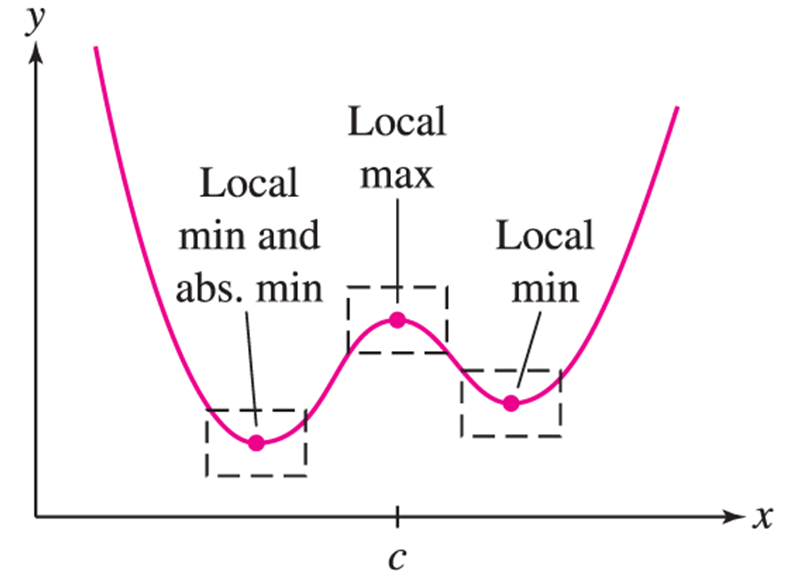
\includegraphics[width=2.5in]{11-09P_locminmax.png}
        \end{center}
\end{definition}

We will spend a good amount of time in the future \textbf{finding} and \textbf{classifying} these local extrema.

\begin{theorem}[Fermat's Theorem on Local Extrema]
        If $f(c)$ is a local max or min, then $c$ is a \textbf{critical point} of $f$:
        either $f'(c) = 0$ or $f'(c)$ DNE.
        \begin{center}
                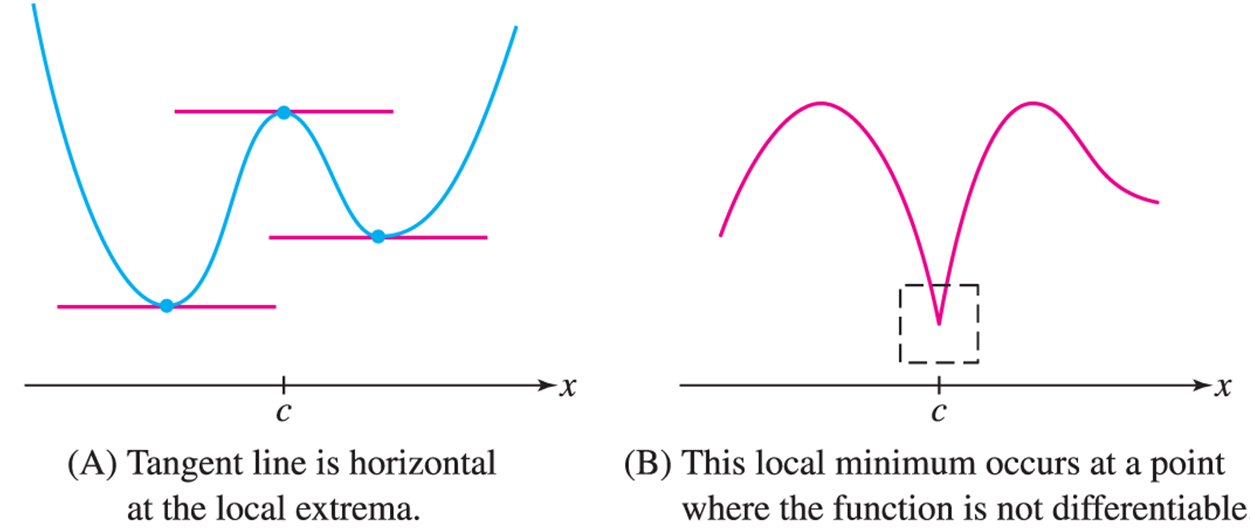
\includegraphics[width=4in]{11-09P_cp.png}
        \end{center}
\end{theorem}

Thus we should think of \textbf{critical points} as \textit{potential local extrema}.

\newpage

\begin{exercise}
        Find the critical points and the associated function values for:
        \begin{enumerate}[(a)]
        \item $f(x) = x^2 - 2x+4$
                \vfill
        \item $f(x) = x^{-1} - x^{-2}$
                \vfill
        \item $f(x) = |2x+1|$
                \vfill                
        \end{enumerate}
\end{exercise}

\newpage

\section{Absolute Extrema}

\begin{definition}
        Let $f$ be a function defined on an interval $I$, and let $a$ be in $I$. We say that $f(a)$ is the
        \begin{itemize}
        \item \textbf{absolute minimum} of $f$ on $I$ if $f(a) \leq f(x)$ for all $x$ in $I$
        \item \textbf{absolute maximum} of $f$ on $I$ if $f(a) \geq f(x)$ for all $x$ in $I$
        \end{itemize}
\end{definition}

\begin{example}
        Not every function has an absolute max or min:
        \begin{itemize}
        \item The function $f(x) = x$ on $(-\infty,\infty)$ increases without bound as $x \to \infty$, and descreases without bound as $x \to -\infty$
        \item If $f$ is \textbf{discontinuous} or defined on an \textbf{open interval}, it need not achieve a max value or a min value
        \end{itemize}
        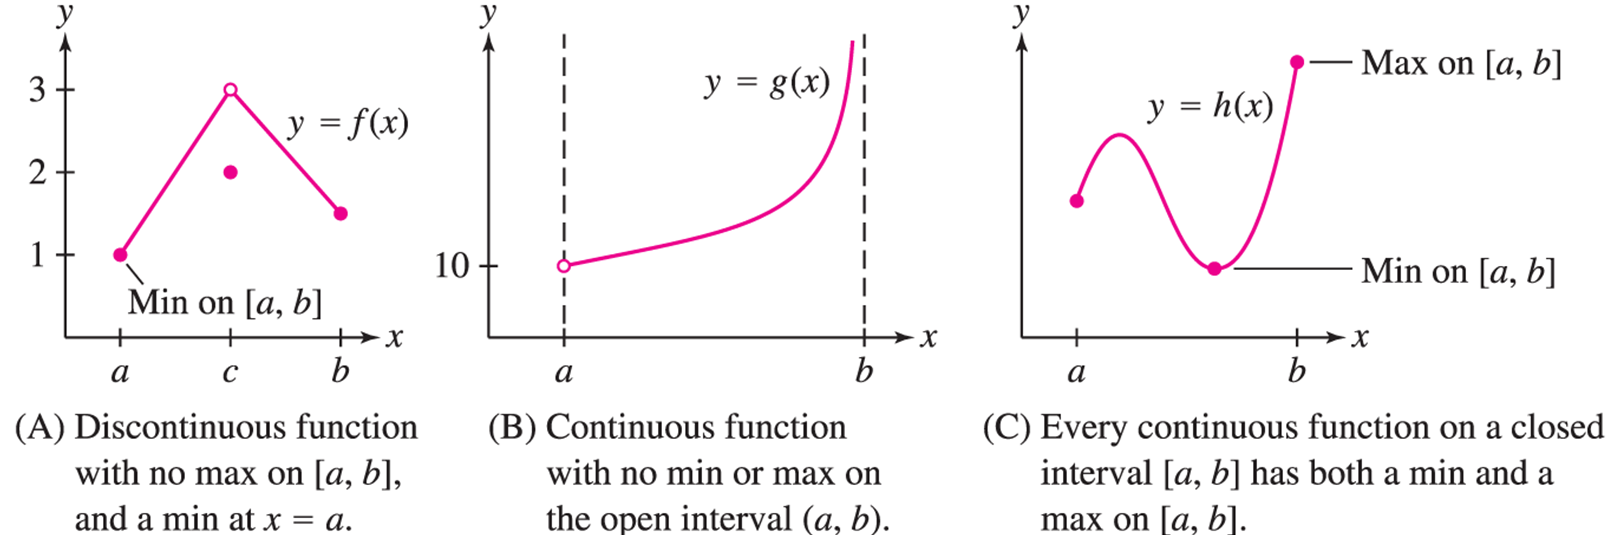
\includegraphics[width=\textwidth]{11-09P_ext.png}
\end{example}

\begin{theorem}[Extreme Value Theorem on a Closed Interval]
        If $f$ is continous on closed interval $I = [a,b]$, that $f$ acheives both an absolute max and an absolute min on $[a,b]$.
        Moreover, these occur at either \textit{critical points} or the \textit{endpoints} $a,b$.
\end{theorem}

\begin{exercise}
        Find the absolute extreme values of $f(x)$ on the interval given
        by comparing values at the critical points and endpoints:
        \begin{enumerate}[(a)]
        \item $f(x) = x^2 - 2x + 4$, $I = [0,2]$
                \vfill
        \item $f(x) = x^{-1} - x^{-2}$, $I = [0,4]$
                \vfill
        \item $f(x) = |2x+1|$, $I = [1,3]$
                \vfill
        \end{enumerate}
\end{exercise}

\newpage

\begin{theorem}[Rolle's Theorem]
        Suppose $f$ is continuous on $[a,b]$ and differentiable on $(a,b)$.
        If $f(a) = f(b)$, then there exists a number $c$ between $a$ and $b$ such that $f'(c) = 0$.
\end{theorem}
 
\begin{exercise}
        Verify Rolle's Theorem for $f(x) = \sin(x)$ on $[\pi/4,3\pi/4]$:
        check that $f(a) = f(b)$, and find the value $c$ in $(\pi/4,3\pi/4)$ such that $f'(c) = 0$.
        \vfill
\end{exercise}

\begin{exercise}
        Use Rolle's Theorem to prove that $f(x) = x^3+3x^2+6x$ has precisely one real root:
        \begin{enumerate}[(a)]
        \item Find points $x = a$ and $x=b$ such that $f(a) < 0$ and $f(b) > 0$.
                \vfill
        \item By the \textbf{Intermediate Value Theorem}, there thus exists some point $c$ in $(a,b)$ with $f(c) = 0$, so
                $f(x)$ has at least one real root.
                (We do not need to find the exact value of $x=c$.)
        \item By Rolle's Theorem, what would have to be true about $f$ if it had another root at $x=d$?
                \vfill
        \item Why is the above not possible?
                \vfill
        \end{enumerate}
\end{exercise}

\newpage

\begin{exercise}
        Find the absolute extreme values of $f(x)$ on the interval given
        by comparing values at the critical points and endpoints:
        \begin{enumerate}[(a)]                
        \item $f(x) = \dfrac{x^2+1}{x-4}$, $I = [5,6]$.
                \vfill
        \item $f(x) = x + \sin x$, $I = [0, 2\pi]$
                \vfill
        \item $f(x) = \dfrac{\ln x}{x}$, $I = [1,3]$
                \vfill
        \end{enumerate}
\end{exercise}

\end{document}
